\chapter{Hello World}
\section{Providerwahl}
Wir haben uns für Swisscom als Provider entschieden, da es uns wichtig war, einen lokalen, heimischen Anbieter gezüglich Cloud Computing besser kennenzulernen. Swisscom ist in vielen Bereichen der IT und Telekommunikation schweizweit marktführend. 

In einem Gastvortrag an der HSR im Herbst 2016 ist ein Vertreter der Swisscom erschienen und hat von der Vorzügen und der gelebten Swissness erzählt. Da wir noch nie mit PaaS Produkten im Allgemeinen gearbeitet haben war dies die perfekte Möglichkeit um in die Thematik reinzufinden. 
\section{Anleitung}
Der Einstieg fiel allgemein gesehen leicht. Swisscom verwendet \glqq Cloud Foundry\grqq für ihre Application Cloud. Mittels Tutorials auf der Webseite wird man für den Einstieg gut \glqq an der Hand genommen\grqq .

\begin{longtable}{| p{5cm} | p{11cm} |}
\hline
Unter https://docs.developer.swisscom.com/getting-started/ 
findet man Tutorials für die verschiedenen PaaS Produkte wie z.B. Python, Java, Node.js
&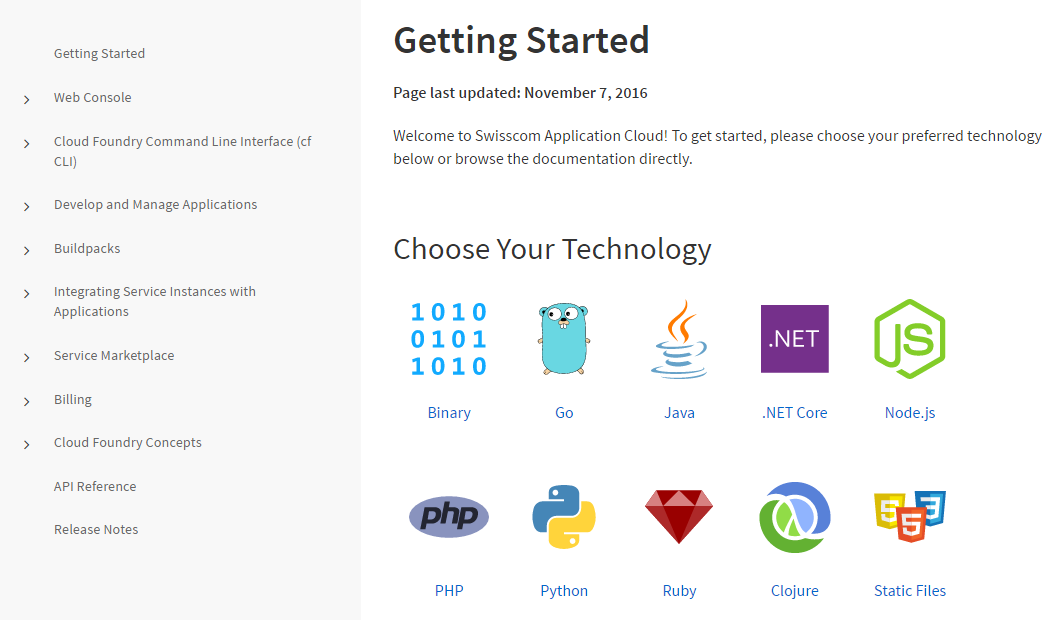
\includegraphics[width=0.65\columnwidth, valign=T]{images/image1.png}\\ \hline
Als allererstes benötigt man das Cloud Foundry Command Line Interface. Auf der Webseite sind Beschreibungen für die Installation unter Linux/Macintosh/Windows zu finden. (Windows in dieser Anleitung) 
&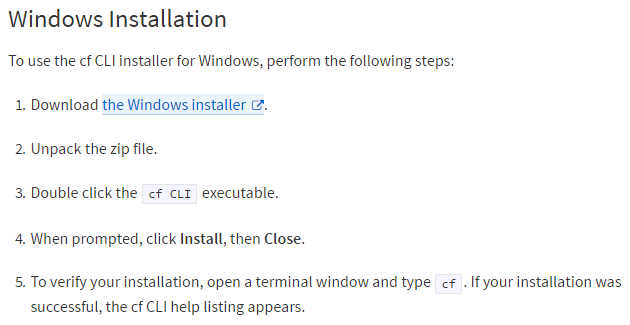
\includegraphics[width=0.65\columnwidth, valign=T]{images/image2.png} \\ \hline
Nach erfolgreicher Installation ist das „cf“-Tool per Windows Commandline (cmd) benutzbar&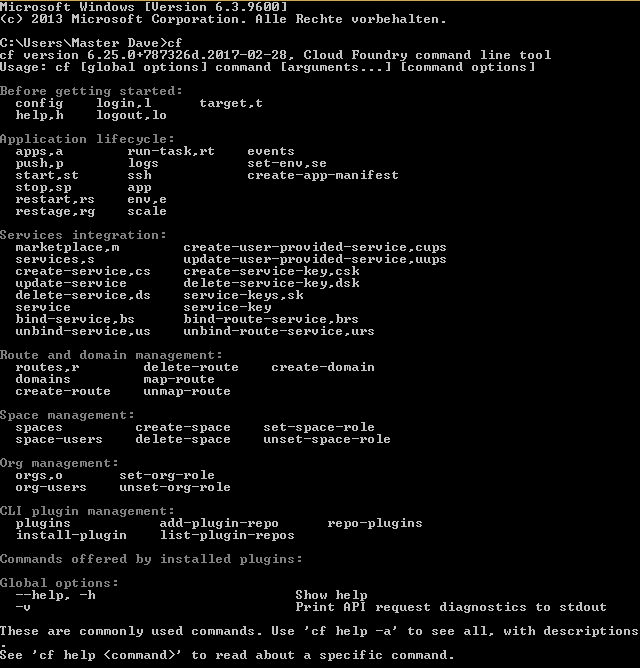
\includegraphics[width=0.65\columnwidth, valign=T]{images/image3.png} \\ \hline
Nun können wir uns mit der Web Console von der Swisscom App Cloud vertraut machen. Auch hier gibt es ein Tutorial 
&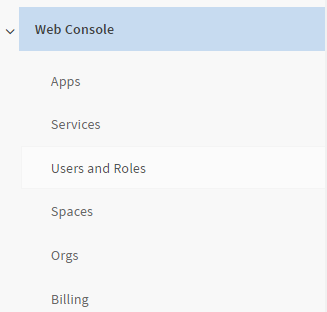
\includegraphics[width=0.65\columnwidth, valign=T]{images/image4.png} \\ \hline
Jetzt können wir das Tutorial für eine Java App durcharbeiten &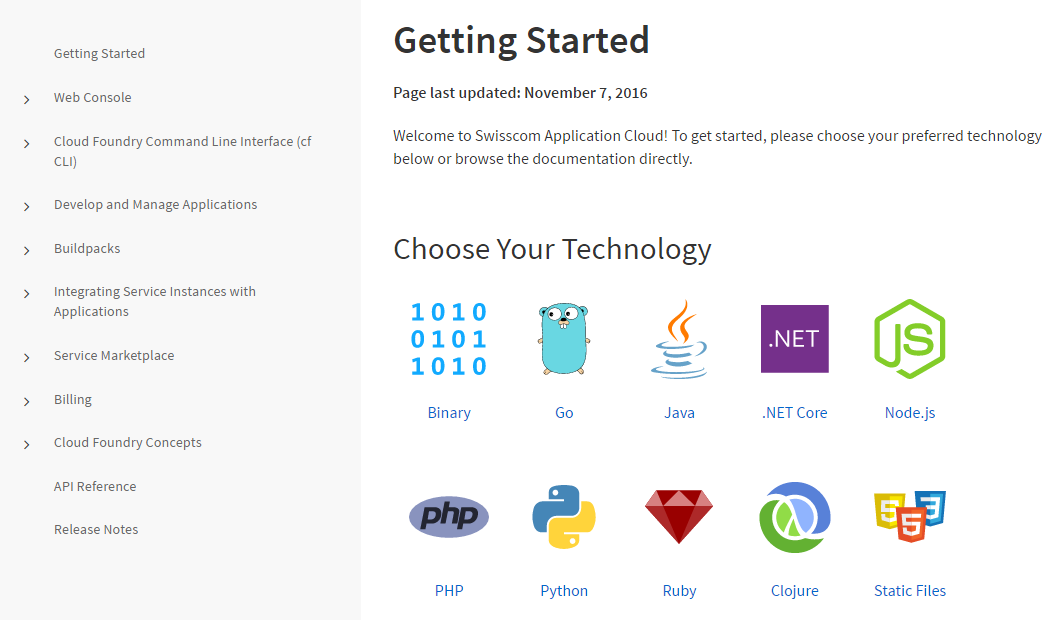
\includegraphics[width=0.65\columnwidth, valign=T]{images/image1.png} \\ \hline
Als Erstes sollte man die Prereqs überprüfen 
&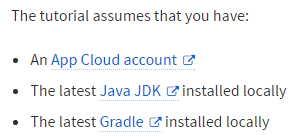
\includegraphics[width=0.65\columnwidth, valign=T]{images/image5.png} \\ \hline
Nun muss man sich über die cf Console an der Swisscom App Cloud anmelden. Wir skippen die Zuweisung an eine Org. 
&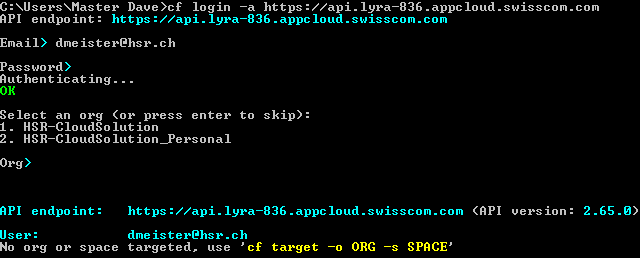
\includegraphics[width=0.65\columnwidth, valign=T]{images/image6.png} \\ \hline
Unter https://console.developer.swisscom.com erstellen wir eine neue Org Namens „HelloWorld“. &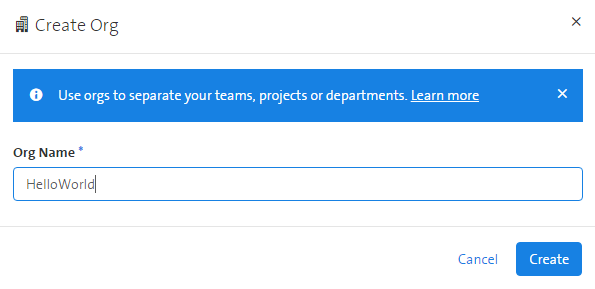
\includegraphics[width=0.65\columnwidth, valign=T]{images/image7.png} \\ \hline
In dieser Org müssen wir einen Space erstellen. 
&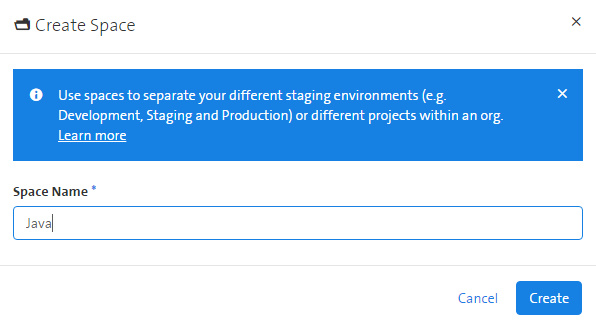
\includegraphics[width=0.65\columnwidth, valign=T]{images/image8.png} \\ \hline
Wir weisen nun Org und Space mittels „cf target –o HelloWorld –s Java“ zu &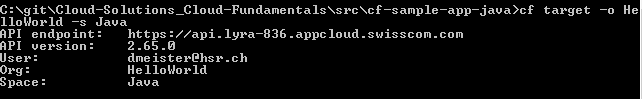
\includegraphics[width=0.65\columnwidth, valign=T]{images/image9.png} \\ \hline
Wir kopieren nun die Java Beispielapp von Swisscom 
&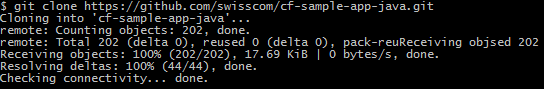
\includegraphics[width=0.65\columnwidth, valign=T]{images/image10.png} \\ \hline
Nun können wir mit Gradle die App builden. Es wurde ein jar generiert. &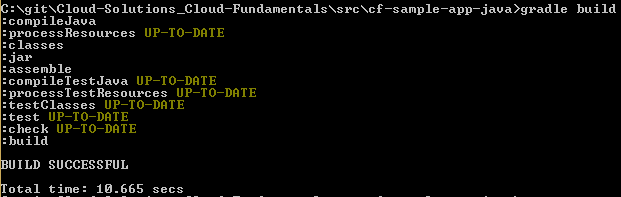
\includegraphics[width=0.65\columnwidth, valign=T]{images/image11.png} \\ \hline
Diese .jar File können wir nun mittels „cf push my-java-app“ –p <path to jar>„ –n „ pushen &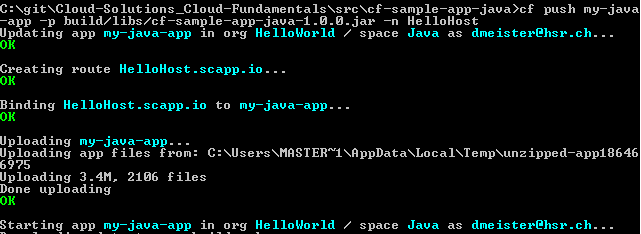
\includegraphics[width=0.65\columnwidth, valign=T]{images/image12.png} \\ \hline
Sobald die App erfolgreich gestartet wurde erscheinen folgende Meldungen &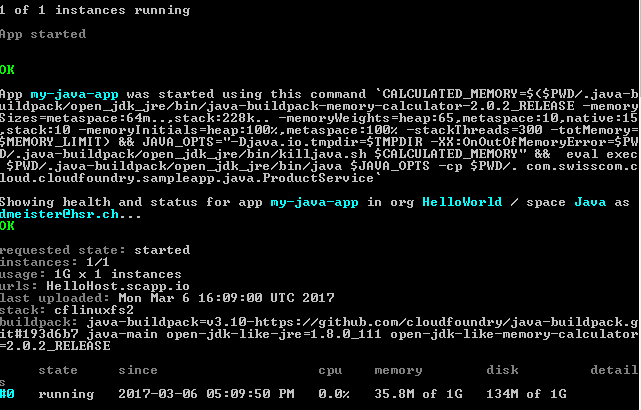
\includegraphics[width=0.65\columnwidth, valign=T]{images/image13.png} \\ \hline 
Mittels „cf app my-java-app“ kann man den Status der Java App abrufen &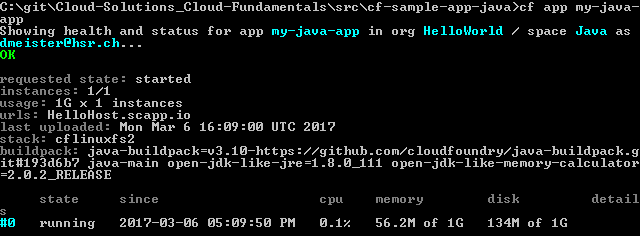
\includegraphics[width=0.65\columnwidth, valign=T]{images/image14.png} \\ \hline
Mittels „cf scale my-java-app“ erhält man eine Übersicht über die verwendeten Ressourcen Memory, Disk, Instances 
&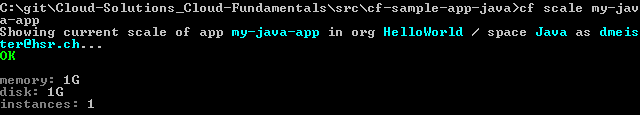
\includegraphics[width=0.65\columnwidth, valign=T]{images/image15.png} \\ \hline
Horizontales Scaling geschieht mittels „cf scale my-java-app –i 3“. So werden nun 3 Instanzen verwendet 
&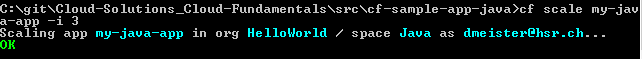
\includegraphics[width=0.65\columnwidth, valign=T]{images/image16.png} \\ \hline
Vertikales Scaling geschieht mittels „cf scale my-java-app –m 2G“. So werden 2 GB RAM verwendet &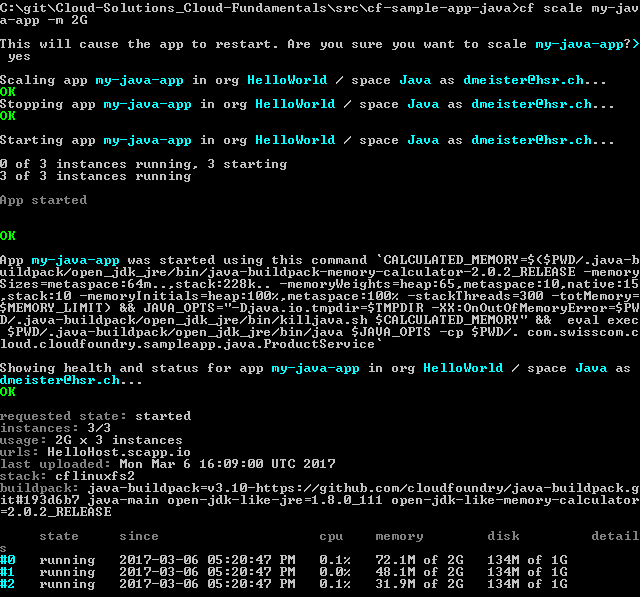
\includegraphics[width=0.65\columnwidth, valign=T]{images/image17.png} \\ \hline
Es gilt nun zu beachten, dass nach dem Scaling die Betriebskosten gestiegen sind. &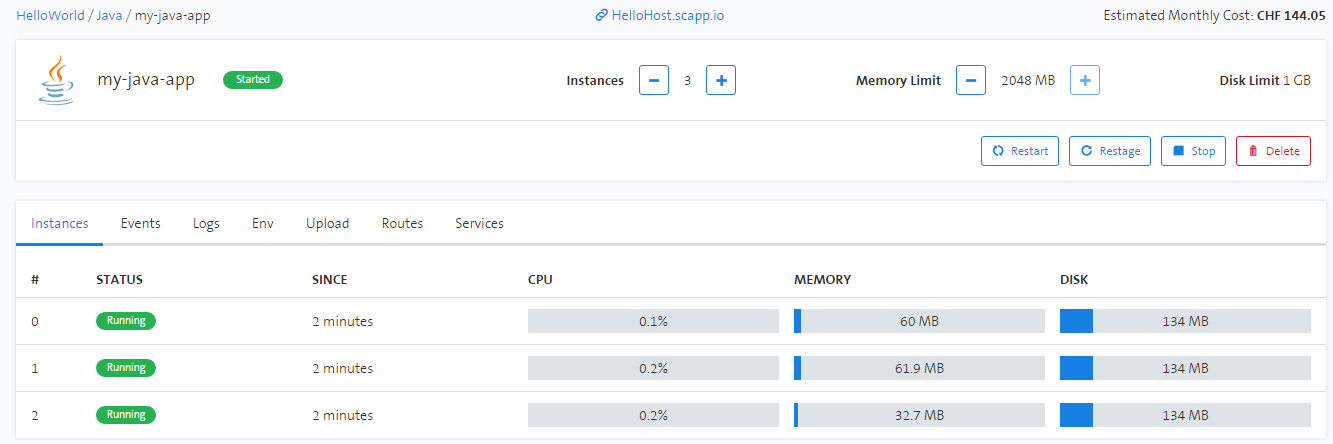
\includegraphics[width=0.65\columnwidth, valign=T]{images/image18.png} \\ \hline
Die Logfiles können einfach mittels „cf logs my-java-app --recent“ abgerufen werden &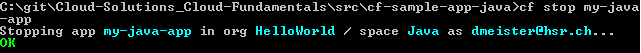
\includegraphics[width=0.65\columnwidth, valign=T]{images/image19.png} \\ \hline
Mittels „cf stop my-java-app“ kann die App gestoppt werden. Falls sie wieder benötigt wird kann sie mittels „cf start my-java-app“ wieder hochgefahren werden. 
&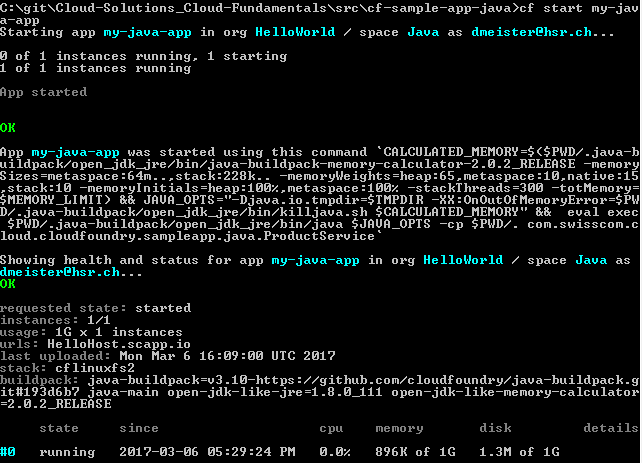
\includegraphics[width=0.65\columnwidth, valign=T]{images/image20.png} \\ \hline
\end{longtable}

\section{Vergleich mit der Google App Engine}
Datenhaltung in der Schweiz, usw. blablabla

\chapter{OSSM-Definition}
\chapter{Cloud Computing Patterns}
\chapter{Self-Information}
\chapter{Preisrecherche}
\chapter{Preisvergleich Hosting vs IaaS vs PaaS}
\chapter{Twelve-Factor Apps}

